\documentclass[a4paper,11pt]{article}
\pdfoutput=1 % if your are submitting a pdflatex (i.e. if you have
             % images in pdf, png or jpg format)

\usepackage{jheppub} % for details on the use of the package, please
                     % see the JHEP-author-manual

\usepackage[T1]{fontenc} % if needed
\usepackage{multirow}
\usepackage{graphicx}
\usepackage{xspace} %load xspace

\usepackage{bookmark} % helps booksmarks look better in PDF
%hypersetup option 'breaklinks' is reguired for line wrapping in the table of contents during latex compilation, and can be removed if you use pdflatex
\hypersetup{colorlinks=true,linkcolor=blue, breaklinks} %internal links in blue, citations in green
%\hypersetup{colorlinks=true,linkcolor=black, citecolor=black, breaklinks} %all links in black
\usepackage[all]{hypcap}

%Use of natbib is STRONGLY recommended to sort and compress your references within each citation
%With these options, natbib will convert i.e. [5,3,9,4] to [3-5, 9]
%\usepackage[sort&compress]{natbib}
%\usepackage[nottoc,numbib]{tocbibind}
%\usepackage{cite}

%%%%%%%%%%%%%%%%%%%%%%%%% Custom Commands/Environments %%%%%%%%%%%%%%%%%%%%%%%%%
% Put your favorite custom commands here
%A list of shortcuts I intend to use
%Only those used will be displayed, so you can just add to this list

% +--------------------------------------------------------------------+                                                                                                                                                                    
% |  Useful miscellaneous things                                       |                                                                                                                                                                      
% +--------------------------------------------------------------------+                                                                                                                                          
\newcommand\quotebox[1]{\parbox{.7\textwidth}{#1}}
\newcommand{\ttH}{\ensuremath{t\bar{t}H}\xspace}

% +--------------------------------------------------------------------+                                                                                                                                                                    
% |  Useful things for W-helicity physics                           |                                                                                                                                                                      
% +--------------------------------------------------------------------+                                                                                                                                                                    
%\newcommand*{\w}{\ensuremath{W}\xspace}
\newcommand*{\w}{\ensuremath{W}\xspace}
\newcommand*{\bt}{\ensuremath{b}\xspace}
\newcommand*{\fo}{\ensuremath{F_{\text{0}}}\xspace}
\newcommand*{\fl}{\ensuremath{F_{\text{L}}}\xspace}
\newcommand*{\fr}{\ensuremath{F_{\text{R}}}\xspace}
\newcommand*{\Wtb}{\ensuremath{Wtb}\xspace}
\newcommand{\ttbar}{\ensuremath{t\bar{t}}\xspace}

% +--------------------------------------------------------------------+                                                                                                                                                                    
% |  Useful things for dihiggs physics                           |                                                                                                                                                                      
% +--------------------------------------------------------------------+                                                                                                                                                                    
%\newcommand*{\w}{\ensuremath{W}\xspace}
\newcommand*{\mbb}{\ensuremath{m_{b\bar{b}}}\xspace}
%\newcommand*{\dsig}{\ensuremath{|\sigma_{d_{0}}|}\xspace}
\newcommand*{\dsig}{\ensuremath{|d_{0}/\sigma_{d_{0}}|}\xspace}
\newcommand*{\ptbb}{\ensuremath{p_{\text{T}}^{b\bar{b}}}\xspace}
\newcommand*{\ptww}{\ensuremath{p_{\text{T}}^{WW}}\xspace}
\newcommand*{\drbb}{\ensuremath{\Delta\text{R}_{b\bar{b}}}\xspace}
\newcommand*{\drww}{\ensuremath{\Delta\text{R}_{WW}}\xspace}
\newcommand*{\mww}{\ensuremath{\text{m}_{WW}}\xspace}
\newcommand*{\mhh}{\ensuremath{\text{m}_{hh}}\xspace}
\newcommand*{\mtw}{\ensuremath{\text{m}_{\text{T}}^{W}}\xspace}
\newcommand*{\bbWW}{\ensuremath{\lowercase{b\bar{b}}WW^*}\xspace}
\newcommand{\bbbar}{\ensuremath{b\bar{b}}\xspace}

% +--------------------------------------------------------------------+                                                                                                                                                                   
% | Masses                                                             |                                                                                                                                                                   
% +--------------------------------------------------------------------+                                                                                                                                                                    
\newcommand*{\mh}{\ensuremath{m_{h}}\xspace}
\newcommand*{\mW}{\ensuremath{m_{W}}\xspace}
\newcommand*{\mZ}{\ensuremath{m_{Z}}\xspace}
\newcommand*{\mH}{\ensuremath{m_{H}}\xspace}
\newcommand*{\mt}{\ensuremath{m_{t}}\xspace}
\newcommand*{\mb}{\ensuremath{m_{b}}\xspace}

% +--------------------------------------------------------------------+                                                                                                                                                           
% |                                                                    |                                                                                                                                                                 
% |  e+e-, etc.                                                        |                                                                                                                                                                 
% |                                                                    |                                                                                                                                                                   
% +--------------------------------------------------------------------+                                                                                                                                                                    
\newcommand*{\ee}{\ensuremath{e^{+} e^{-}}\xspace}
\newcommand*{\epm}{\ensuremath{e^{\pm}}\xspace}
\newcommand*{\epem}{\ensuremath{e^{+} e^-}\xspace}
\newcommand*{\mumu}{\ensuremath{\mu^{+} \mu^{-}}\xspace}
\newcommand*{\tautau}{\ensuremath{\tau^{+} \tau^{-}}\xspace}
\newcommand*{\leplep}{\ensuremath{\ell^{+} \ell^{-}}\xspace}
\newcommand*{\ellell}{\ensuremath{\ell^{+} \ell^{-}}\xspace}
\newcommand*{\lnu}{\ensuremath{\ell \nu}\xspace}

% +--------------------------------------------------------------------+                                                                                                                                                      
% |                                                                    |                                                                                                                                                
% |  Vector bosons                                                     |                                                                                                                                                           
% |                                                                    |                                                                                                                                                        
% +--------------------------------------------------------------------+                                                                                                                                                                    
\newcommand*{\Zzero}{\ensuremath{Z}\xspace}
\newcommand*{\Zboson}{\ensuremath{Z}\xspace}
\newcommand*{\Wplus}{\ensuremath{W^{+}}\xspace}
\newcommand*{\Wminus}{\ensuremath{W^{-}}\xspace}
\newcommand*{\Wboson}{\ensuremath{W}\xspace}
\newcommand*{\Wpm}{\ensuremath{W^{\pm}}\xspace}
\newcommand*{\Wmp}{\ensuremath{W^{\mp}}\xspace}

% +--------------------------------------------------------------------+                                                                                                                                                                 
% |  Useful things for proton-proton physics                           |                                                                                                                                                                  
% +--------------------------------------------------------------------+                                                                                                                                                                    
\newcommand*{\pT}{\ensuremath{p_{\text{T}}}\xspace}
\newcommand*{\pt}{\ensuremath{p_{\text{T}}}\xspace}
\newcommand*{\ET}{\ensuremath{E_{\text{T}}}\xspace}
\newcommand*{\eT}{\ensuremath{E_{\text{T}}}\xspace}
\newcommand*{\et}{\ensuremath{E_{\text{T}}}\xspace}
\newcommand*{\HT}{\ensuremath{H_{\text{T}}}\xspace}
\newcommand*{\pTsq}{\ensuremath{p_{\text{T}}^{2}}\xspace}
%\newcommand*{\ptsq}{\ensuremath{p_{\text{T}}^{2}}\xspace}                                                                                                                                                                       
\newcommand*{\MET}{\ensuremath{E_{\text{T}}^{\text{miss}}}\xspace}
\newcommand*{\met}{\ensuremath{E_{\text{T}}^{\text{miss}}}\xspace}
\newcommand*{\sumET}{\ensuremath{\sum \ET}\xspace}
\newcommand{\EjetRec}{\ensuremath{E_{\text{rec}}}}
\newcommand{\PjetRec}{\ensuremath{p_{\text{rec}}}}
\newcommand{\EjetTru}{\ensuremath{E_{\text{truth}}}}
\newcommand{\PjetTru}{\ensuremath{p_{\text{truth}}}}
\newcommand{\EjetDM}{\ensuremath{E_{\text{DM}}}}
\newcommand{\Rcone}{\ensuremath{R_{\text{cone}}}}
\newcommand*{\abseta}{\ensuremath{|\eta|}\xspace}
\newcommand*{\Ecm}{\ensuremath{E_{\text{cm}}}}
\newcommand*{\rts}{\ensuremath{\sqrt{s}}\xspace}
\newcommand*{\sqs}{\ensuremath{\sqrt{s}}\xspace}
\newcommand*{\Nevt}{\ensuremath{N_{\mathrm{evt}}}\xspace}
\newcommand*{\zvtx}{\ensuremath{z_{\mathrm{vtx}}}\xspace}
\newcommand*{\dzero}{\ensuremath{d_{0}}\xspace}
\newcommand*{\zzsth}{\ensuremath{z_{0} \sin(\theta)}\xspace}

%-------------------------------------------------------------------------------
% Useful units. The use of these is deprecated.
% Use a units package, e.g. siunitx instead.
%-------------------------------------------------------------------------------
\newcommand*{\TeV}{\ifmmode {\mathrm{\ Te\kern -0.1em V}}\else
                   \textrm{Te\kern -0.1em V}\fi}%
\newcommand*{\GeV}{\ifmmode {\mathrm{\ Ge\kern -0.1em V}}\else
                   \textrm{Ge\kern -0.1em V}\fi}%
\newcommand*{\MeV}{\ifmmode {\mathrm{\ Me\kern -0.1em V}}\else
                   \textrm{Me\kern -0.1em V}\fi}%
\newcommand*{\keV}{\ifmmode {\mathrm{\ ke\kern -0.1em V}}\else
                   \textrm{ke\kern -0.1em V}\fi}%
\newcommand*{\eV}{\ifmmode  {\mathrm{\ e\kern -0.1em V}}\else
                   \textrm{e\kern -0.1em V}\fi}%
\let\tev=\TeV
\let\gev=\GeV
\let\mev=\MeV
\let\kev=\keV
\let\ev=\eV

%-------------------------------------------------------------------------------
% Useful miscellaneous things. Mostly baggage from ATLAS defaults
%-------------------------------------------------------------------------------
\newcommand*{\syst}{\mbox{$\;$(syst.)}\xspace}
\newcommand*{\ifb}{\mbox{fb$^{-1}$}} %load list of shortcuts shortcuts.tex
\newcommand{\tab}{\hspace*{2em}}



%%%%%%%%%%%%%%%%%%%%%%%%% Start paper %%%%%%%%%%%%%%%%%%%%%%%%%
\title{\boldmath Learning About Machine Learning With Dihiggs Production at the LHC}

%% %simple case: 2 authors, same institution
%% \author{A. Uthor}
%% \author{and A. Nother Author}
%% \affiliation{Institution,\\Address, Country}

% more complex case: 4 authors, 3 institutions, 2 footnotes
\author[a]{B. Tannenwald}
\author[a]{C. Neu,}
\author[a]{A. Li,}
\author[a]{G. Buehlmann,}
\author[a]{A. Cuddeback,}
\author[a]{R. Parvatam,}
\author[a]{C. Thompson}


% The "\note" macro will give a warning: "Ignoring empty anchor..."
% you can safely ignore it.

\affiliation[a]{University of Virginia, 248 McCormick Road, Charlottesville, VA, USA}

% e-mail addresses: one for each author, in the same order as the authors
\emailAdd{benjamin.tannenwald@cern.sh}
%\emailAdd{christopher.neud@cern.sh}
%\emailAdd{al8fm@virginia.edu}
%\emailAdd{gmb8nj@virginia.edu}
%\emailAdd{atc4yk@virginia.edu}
%\emailAdd{rp5cf@virginia.edu}
%\emailAdd{crt9ag@virginia.edu}


\abstract{Machine learning techniques have started being explored in many new domains of high energy physics analysis. Powerful methods can be used to identify and measure rare processes from previously insurmountable backgrounds. One of the most profound Standard Model signatures still to be discovered at the LHC is the pair production of Higgs bosons through the Higgs self-coupling. The small cross section of this process makes detection very difficult even for the decay channel with the largest branching fraction ($hh\rightarrow b\bar{b}b\bar{b}$). This paper benchmarks a variety of approaches (boosted decision trees, neural networks with straightforward and novel architectures, semi-supervised algorithms) against one another in an attempt to catalogue the various avaiable to high energy physicists as the era of the HL-LHC approaches.}



\begin{document} 
\maketitle
\flushbottom

%%% Main body of paper
\section{Introduction}
\label{sec:intro}

The use of machine learning (ML) techniques in high energy particle physics has rapidly expanded in the last few decades. The proliferation of methods and applications has touched nearly every segment of analysis and reconstruction~\cite{albertsson2018machine} and will be vital in understanding the full dataset of the Large Hadron Collider (LHC) and data from future colliders.

Common approaches involve using linear techniques like decision trees and non-linear approaches like neural networks. These techniques are then used to reconstruct objects like leptons and jets, to tag b-quarks and boosted decays, and to classify different processes. Many models depend on kinematic input features physicists have traditionally used; other architectures rely on emergent features produced in a more abstract phase-space. With so many usable machine-learning options available, interesting questions arise about what types of information are best to feed to our networks. The information that is best for physicists to learn from might not be optimal for sophisticated computing algorithms.
%You can even think of fun semi-supervised approaches like clustering and maybe some stuff with autoencoders. To be totally honest, I'm not really sure if the autoencoder stuff is relevant for this paper, but it's really interesting and is maybe cool for unexpected BSM signatures? Could be a cool side-study.

The goal of this paper is to explore a wide range of current ML techniques that can be used to identify di-Higgs production at the High Luminosity LHC (HL-LHC). Observing di-Higgs production is necessary to measure the self-coupling of the Higgs boson and fully understand the nature of electroweak symmetry breaking. The difficulty in measuring Higgs pair production lies in the tiny cross-section of even the largest branching fraction ($hh\rightarrow b\bar{b}b\bar{b}$) and the relative abundance of similarly reconstructed QCD events.

This paper is organized as follows: Section 2 deals with the physics relevant for di-Higgs production and the QCD background. Sections 3 and 4 summarize the various ML methods tested. The maximum significance
\begin{equation}
  \sigma = \frac{N_{\textrm{signal}}}{\sqrt{N_{\textrm{background}}}}
\end{equation}
is provided for each method along with event yields normalized to the HL-LHC design integrated luminosity of 3000 fb$^{-1}$. Section 5 compares the results from the various approaches.


%\input{defaultContent_1.tex}
%\input{defaultContent_2.tex}

%Dihiggs physics is cool. Also complicated but not that complicated. Mostly just rare. Show some diagrams. Talk about rates.
\section{Di-Higgs Physics}
\subsection{Higgs Pair Production}
\label{sec:physics}

The Higgs boson is an essential part of the Standard Model (SM) of particle physics and is a product of the mechanism responsible for electroweak symmetry breaking. Along with the interaction of the Higgs with the other particles of the Standard Model, the SM predicts the interaction of the Higgs boson with itself at tree-level (self-interaction). This mechanism contributes to non-resonant Higgs boson pair production together with quark-loop contributions via Yukawa-type interactions. Figure~\ref{fig:nr_hh_production} shows a schematic diagram of non-resonant Higgs boson pair production. Since the production cross section for Higgs boson pair production is extremely small within the SM~\cite{deFlorian:2016spz}, 

\begin{equation*}
\sigma_{hh}\text{ (14 TeV)} = 45.1 \text{ fb},
\end{equation*}

any significant deviation would indicate the presence of new physics.

\begin{figure}[!h] 
\begin{center}
\includegraphics*[width=0.75\textwidth] {dihiggsPhys/figures/nr-diHiggs-production.png}
\caption{Leading order Feynman diagrams for non-resonant production of Higgs
  boson pairs in the Standard Model through (a) the Higgs boson self-coupling
  and (b) the Higgs-fermion Yukawa interaction.} 
  \label{fig:nr_hh_production}
\end{center}
\end{figure}

Many extensions of the SM predict the existence of additional scalar bosons which may have mass larger than twice the Higgs mass and can decay into a Higgs boson pair. Searching for resonances in the $hh$ mass spectrum can help us discover or limit exotic models which predict the presence of such particles. More importantly, measuring the SM di-Higgs cross-section (or placing limits on its magnitude) allow us to probe the self-coupling of the Higgs field and better understand the mechanism behind electroweak symmetry breaking.

The following work is focused on techniques for distinguishing non-resonant (SM-like) Higgs boson pair production where both Higgs bosons decay via $h \to b \bar{b}$. The choice of using the $4b$ decay mode provides the largest possible amount of signal events but requires powerful background reduction techniques due to the large production cross-section of fully hadronic QCD processes. All results are quoted for simulated events produced by $pp$ collisions with a center-of-mass energy of 14 TeV and scaled to the full design luminosity of the HL-LHC (an integrated luminosity of 3000 fb$^{-1}$). Simulated samples were produced using ROOT v6.12/04~\cite{Brun:1997pa} and Madgraph v2.7.0~\cite{Alwall:2014hca}. Events were then showered using Pythia v8.2.44~\cite{Sj_strand_2015} and reconstructed with Delphes v3.0~\cite{de_Favereau_2014} using the v2 approximation of the upgraded Phase-II CMS detector.

Both the signal and background samples were generated with minimal pileup addition sampled from a Poisson distribution with an expectation value of zero additional vertices. An additional generator-level cut requiring total hadronic energy greater than 300 GeV was applied when generating background events. All code used to set up the generation environment and produce events is publicly available~\cite{github}. A summary of the sample generation details is shown in Table~\ref{tab:samples}.

\begin{table}[ht!]
 \label{tab:samples}
\centering
  %\begin{center}
    \begin{tabular}{|l|c|c|c|} % <-- Alignments: 1st column left, 2nd middle and 3rd right, with vertical lines in between
      \hline\hline
      Name & Process & $\sigma_{\textrm{eff}}$ [fb] & $N_{\textrm{events}}$ \\
      \hline
      Di-Higgs & $p p > h h$, $h > b \bar{b}$ & 12.4 & 1$\cdot 10^6$ \\
      QCD     & $p p > b \bar{b} b \bar{b}$ & 441866.0 & 4$\cdot 10^6$ \\
      \hline\hline
    \end{tabular}
\caption{Madgraph processes, effective cross-sections, and number of generated events for the signal and background samples used in this paper. The effective cross-sections differ slightly from the total theoretical cross-sections due to branching fractions and generation-level cuts on hadronic activity.}
\end{table}

\subsection{Event Reconstruction}
\label{sec:eventReco}
The first step in reconstructing the 4$b$ system is to reconstruct and select b-jet candidates. Jets are clustered using an anti-$k_T$ algorithm with a radius of R=0.4. To be selected for use in event reconstruction, a jet must have $\pt > 20$ GeV and an absolute value of $\mid\eta\mid < 2.5$. Delphes uses an internal $b$-tagging efficiency parameterization to predict whether jets are tagged, and an event is only fully reconstructed if at least 4 jets are $b$-tagged (unless otherwise specified). The properties and kinematics of selected jets are shown in Fig~\ref{fig:jetInfo}. This strict requirement of having at least 4 $b$-tags in an event helps to reduce contributions from QCD and reduce the combinatoric ambiguity in event reconstruction.

\begin{figure}[ht!]
  \begin{center}
  \subfloat[]{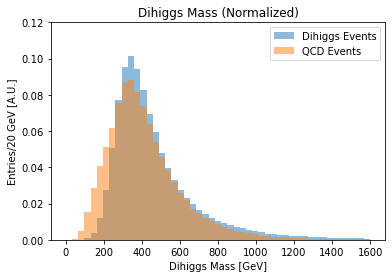
\includegraphics[width = 2in]{dihiggsPhys/figures/recoPlots_08-21-20/dihiggs_DihiggsMass_norm}} 
  \subfloat[]{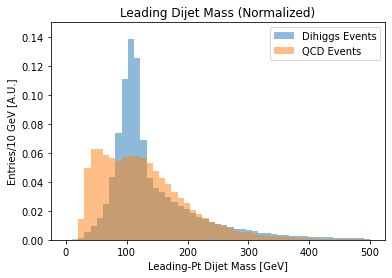
\includegraphics[width = 2in]{dihiggsPhys/figures/recoPlots_08-21-20/leading_Leading-PtDijetMass_norm}}
  \subfloat[]{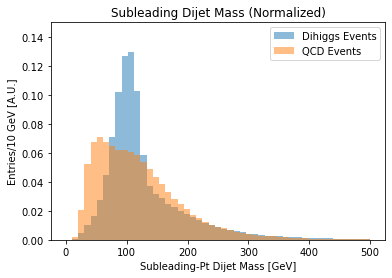
\includegraphics[width = 2in]{dihiggsPhys/figures/recoPlots_08-21-20/subleading_Subleading-PtDijetMass_norm}}\\
  \subfloat[]{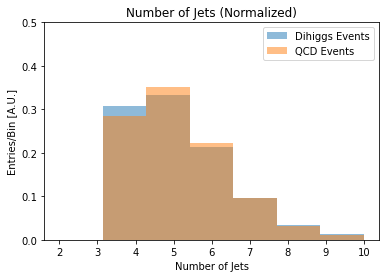
\includegraphics[width = 2in]{dihiggsPhys/figures/recoPlots_08-21-20/number_NumberofJets_norm}}
  \subfloat[]{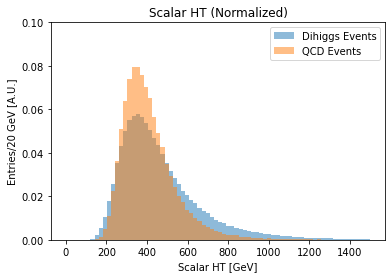
\includegraphics[width = 2in]{dihiggsPhys/figures/recoPlots_08-21-20/scalar_ScalarHT_norm}}
  \subfloat[]{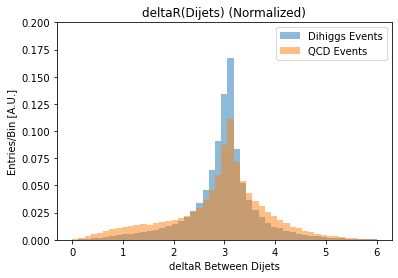
\includegraphics[width = 2in]{dihiggsPhys/figures/recoPlots_08-21-20/deltar(dijets)_deltaRBetweenDijets_norm}} 
  \caption{Sample of event kinematics and reconstructed di-Higgs system from QCD and di-Higgs simulation. Distributions are normalized to the same area to compare shapes.}
  \label{fig:jetInfo}
  \end{center}
\end{figure}

Once events with at least 4 $b$-tags are selected, there is a choice about how to reconstruct the di-Higgs system. Several reconstruction methods were tested for pairing b-jets to find an optimal algorithm for correctly pairing Higgs boson constituents. Two algorithms were selected for use in the following sections: the first iterates through all selected jets in an event and returns the two pairs with closest di-jet masses to one another and the second returns the two jet pairs that minimize the difference between the individual candidate pairs and a Higgs boson mass of 125 GeV. Unless otherwise specified, the method that selects di-jets with masses closest to each other is used when training techniques that require reconstructed events. Fig~\ref{fig:jetInfo} shows a selection of distributions describing the di-Higgs system using this reconstruction algorithm.% Figure~\ref{fig:comapreReco} compares the dijet pair masses obtained from both algorithm. 

%\begin{figure}[ht!]
%  \begin{center}
%  \subfloat[]{\includegraphics[width = 2.5in]{dihiggsPhys/figures/reconstructedQuantities/mh_pairJetsUsingSmallestDeltaR}} 
%  \subfloat[]{\includegraphics[width = 2.5in]{dihiggsPhys/figures/reconstructedQuantities/mh_pairJetsClosestToHiggs}}\\
%  \caption{Leading dijet mass using different reconstruction algorithms. Left plot shows mass when minimizing dijet angular separation, right plot shows mass when minimizing different between dijet mass and a Higgs mass of 125 GeV ('closestDijetMassToHiggs'). [PLACEHOLDER PLOTS]}
%  \label{fig:compareReco}
%  \end{center}
%\end{figure}

Reconstructed variables include the masses and momentum of the four- and two-body Higgs candidates as well as the angular separations between the two Higgs candidates and their constituent jets. Additional event-level variables like the number of selected jets, the number of b-tagged jets, and the missing transverse energy in the event were also considered as inputs to various algorithms. All possible variables were evaluated using the Kolmogorov-Smirnov (KS) test for individual separation power between signal and background. Variables were sorted in descending order of KS separability. Each algorithm is trained on a subset that balances minimizing the number of variables without sacrificing performance. 


\section{Supervised Learning}
\label{sec:supervised}
Searches for specific signatures or interactions in collider data can be thought of as a classification problem - some known signal process must be identified and separated from some known and well-modeled set of background processes. Any iterative algorithm can then improve its ability to properly identify signal from background by comparing its predicted classifications to the true known classifications and adjusting its internal parameters. This type of approach is known as supervised machine learning, and it is particularly relevant when training models to distinguish between different known processes. We discuss several supervised learning approaches below.

% BDT
\subsection{Boosted Decision Tree}
\label{sec:BDT}
Boosted Decision Trees (BDTs) have a long history in high energy physics from enabling the first observation of single top production at the Tevatron~\cite{Abazov:2006gd, Aaltonen:2008sy} to helping in the discovery of the Higgs boson at the LHC~\cite{Aad_2012, Chatrchyan_2012}. A decision tree functions by making a series of cuts (or decisions) that maximize the separation between signal and background events in a single dimension. Each cut produces a branch in the tree containing independent populations. The depth of the tree sets the number of decisions a tree will make, and a well-designed tree will have end-nodes that efficiently separate and properly identify the constituent classes. Any series of cuts for identifying events will inevitably misclassify some events, and there are many strategies for improving the results. A boosted decision tree attempts to improve the classification by creating a new set of data from the improperly classified events and training a new decision tree on these inputs. Each step of re-training with misclassified events is called a \textit{boost}, and the total prediction for an event is the weighted sum of predictions from the orignal tree and the boosted trees where each sequential boost recieves a smaller weight in the sum.

The BDT trained for di-Higgs detection was built using the xgboost package~\cite{xgboost}. The top seventeen reconstructed and event-level variables ranked by KS separability (discussed in Section~\ref{sec:eventReco}) were used in training. The hyperparameters describing the boosted decision tree were optimized for maximum $S/\sqrt{B}$. The optimal hyperparamters were found to be as follows: multiplicative boost factor of 0.1, maximum tree depth of 9, gamma (minimum loss reduction needed for further partition) of 1.1, and an L2 regularization term of 8.28.

\begin{figure}[!h]
\begin{center}
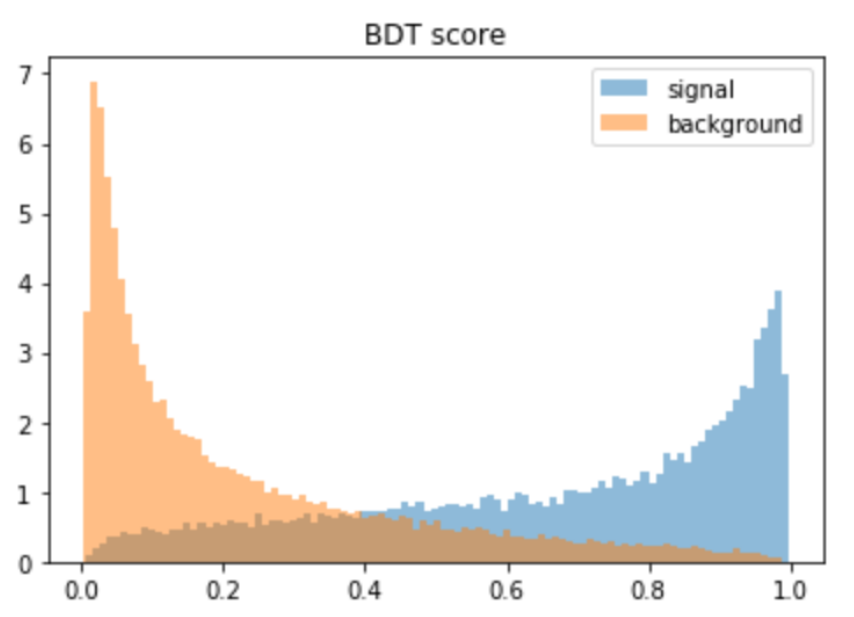
\includegraphics[width=3in]{BDT/bdt_pred}
\caption{Signal predictions of the trained BDT for signal and background samples independent from the training sets.}
\label{fig:bdt_pred}
\end{center}
\end{figure}

The predictions from the optimized BDT are shown in Figure~\ref{fig:bdt_pred}. A maximum significance of 1.84$\pm$0.09 was obtained, yielding 986 signal events and 2.8$\cdot 10^5$ background events. 


% BDT
\subsection{Random Forest}
\label{sec:RandomForest}
Random Forest algorithms share a similar tree structure with BDTs, but they leverage ensembles of independent decision trees as opposed to iteratively improving the predictions of a single tree using mis-classified events. Each tree in a random forest is `grown` using a random sampling of input variables and training events. The randomness of the sampling ensures each tree yields a unique but correlated prediction compared to the other trees in the forest. The class prediction of the forest is the majority vote of the constituent trees. Tuning the hyperparameters of a random forest requires optimizing the number of trees in the forest, the sub-sampling used to produce each tree, as well as more familiar decision tree parameters like child depth. 

The random forest trained for dihiggs classification uses the ‘closestDijetMassToHiggs’ reconstruction algorithm and samples from the top seventeen reconstructed kinematic and event-level variables. The input variables were selected as having the highest separability between dihiggs and QCD processes. The random forest was implemented using the 'XGBRFClassifier` functionality from xgboost~\cite{xgboost}. Detail the hyperparameters. Predictions were made on data fully independent from the training data, and the results are shown in Figure~\ref{fig:rf_score}

\begin{figure}[!h] 
\begin{center}
\includegraphics*[width=0.75\textwidth] {randomForest/figures/rf_score.png}
\caption{Output score on the testing dataset with the fully trained random forest classifier.}
  \label{fig:rf_score}
\end{center}
\end{figure}

The best significance for the random forest approach is found to be $S/\sqrt{B}$ = 2.17$\pm$0.22 when requiring a prediction score > 0.81. 


% ff Neural Network
\subsection{Feed Forward Neural Network}
\label{sec:NN}
Fully connected or feed-forward neural networks (NNs) also have a long history in high energy physics. The fundamental element of any neural network is called a \textit{layer}. Multiple layers are stacked together to produce a final prediction given the input variables from the first layer. This predicted outcome is then evaluated against a known target value. A fully-connected network can have multiple internal (or hidden) layers between the input and output layers, and each hidden layer is composed of a series of trainable activation functions and weights that allow the network to identify and iteratively combine important features of the input space. A function (called the loss function) is chosen to quantify the difference between the model prediction and target values. The loss calculated after a single training iteration is used to adjust the internal network weights in the next training iteration through a process called backpropagation. The model is fully trained once the improvement in the loss between iterations falls beneath some user-defined threshold.

The NN trained for di-Higgs detection was built using the Keras~\cite{chollet2015keras} and Tensorflow~\cite{tensorflow} packages. The top twenty-two most separable reconstructed and event-level variables were used as the input variables for the NN. The complete network structure consists of the input layer, two hidden layers, and a single-node output layer. The first hidden layer contains 175 nodes with an L2 kernel regularizer ($\lambda$ = $10^{-4}$). The second hidden layer contains 90 nodes with no kernel regularizer. A batch normalization layer and a dropout (0.2) function are placed in between the two hidden layers to prevent over-fitting. Both hidden layers use a rectified linear (ReLU) activation function, while the output layer uses a sigmoid activation function. Several models were trained by individually tuning each hyperparameter over a reasonable range in order to produce a final optimized model. A schematic flowchart of the network structure is shown in Figure~\ref{fig:nn}.
%The sequential model was compiled using the ‘adam’ optimizer along with the ‘binary\_crossentropy’ loss method. Finally, the model was fit on the training data along with the validation data for 100 epochs. 

\begin{figure}[!h] 
\begin{center}
\includegraphics*[width=0.75\textwidth] {ffNN/figures/flowchart_ffNN.png}
\caption{Structure of the feed-forward neural network. The input variables are fed through two fully connected dense layers to classify events. One dropout layer and one batch normalization layer help mitigate over-fitting during training.}
  \label{fig:nn}
\end{center}
\end{figure}

The NN was trained for 25 epochs before the minimal loss-improvement threshold was met, and the results are shown in Figure~\ref{fig:results_nn}. The trained model obtained a maximum $\sigma$ = 2.40$\pm$0.08 when considering events with a signal prediction score > 0.94. This phase-space has a signal yield of $1659.9 \pm 12.5$ events and a background yield of $4.8 \pm 0.2$ $\cdot$ $10^5$ events. %477215.3 events.

\begin{figure}[!h] 
\begin{center}
   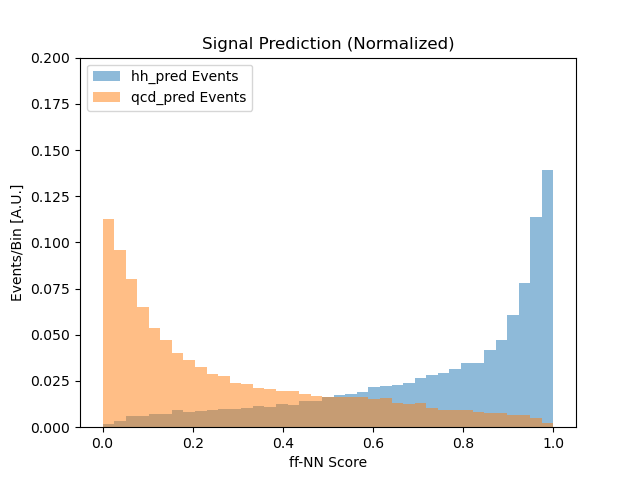
\includegraphics[width = 3in]{ffNN/figures/score_ffnn_v3}\\
\caption{Final predictions of the feed-forward network for signal and background samples.}
  \label{fig:results_nn}
\end{center}
\end{figure}



% ff Neural Network
\subsection{Convolutional Neural Network}
\label{sec:CNN}
Convolutional Neural Networks (CNNs) are neural networks that predict the content of an input image by using assumptions about the local relationships between neighboring pixels. For this analysis, content prediction is simplified to a general classification of whether the image comes from a di-Higgs or QCD event. The fundamental elements of any convolutional network are convolutional layers and pooling layers. Convolutional layers use filters that perform linear combinations of neighboring pixels within the filter size, and pooling layers aggregate information by grouping neighboring pixels using either their maximum or average values. After some number of these layers, the output is flattened into a one-dimensional vector, and this flattened vector is pushed through a set of feed-forward layers in order to make a final output prediction. 

Many previous papers have explored the use of convolutional networks trained on low-level quantities (e.g. tracks and calorimeter deposits) for the purposes of object identification~\cite{Alison:2019kud} at colliders. This paper extends the application to event-level identification. Using low-level quantities removes the need to reconstruct higher-level objects like jets or jet pairs; only the detector-level measurements are required for image creation. The performance of four convolutional networks were studied in the context of di-Higgs identification. The first network used a 3-layer image composed of energy/momentum weighted tracks, electromagnetic calorimeter deposits, and hadronic calorimeter deposits. The second network uses the same three layers but appends additional global event-level information to the flattened vector after image processing and before the fully connected layers. Figures~\ref{fig:cnn_nominal} and \ref{fig:cnn_hybrid} depict both network structures. The third and fourth networks follow the same pattern as the previous two but with the addition of two image layers corresponding to longitudinal and transverse impact parameter-weighted track information.

\begin{figure}[!h] 
\begin{center}
\includegraphics*[width=0.75\textwidth] {CNN/figures/nominalCNN.png}
\caption{Structure of the nominal convolutional neural network. The input images are fed through two convolutional layers and a single max-pooling layer before being flattened into a one-dimensional vector. The flattened vector is then fed through one fully connected layer, a batch normalization layer, and a final fully connected layer before a final prediction is made.}
  \label{fig:cnn_nominal}
\end{center}
\end{figure}

\begin{figure}[!h] 
\begin{center}
\includegraphics*[width=0.75\textwidth] {CNN/figures/hybridCNN.png}
\caption{Structure of the hybrid convolutional neural network. The input images are fed through two convolutional layers and a single max-pooling layer before being flattened into a one-dimensional vector. Scaled user-specified variables (e.g. $H_{T}$) are then concatenated with the flattened image vector. The concatenated vector is then fed through one fully connected layer, a batch normalization layer, and a final fully connected layer before a final prediction is made.}
  \label{fig:cnn_hybrid}
\end{center}
\end{figure}

In order to produce coherent images, the center of mass and the center of momentum for each event are calculated. All constituents are then boosted longitudinally into the center of mass of the event and rotated in phi to the center of momentum. After this pre-processing, each image layer corresponds to a 31x31 pixel grid centered on the total activity in the event. Figure~\ref{fig:cnn_avgQCD} shows an average QCD image and Figure~\ref{fig:cnn_avgDihiggs} shows an average di-Higgs image. While the average image layers for each sample closely resemble one another, they do contain different information, and variations are visible.

Importantly, clear differences are observed between the average QCD images and the average di-Higgs images. Each half of the di-Higgs image (split across $\phi$ = 0) is arranged in a roughly circular, isotropic shape due to the spin-0 nature of the Higgs. The QCD images appear balanced because of the effect of the pre-processing, but no similar circular structure is produced. Additionally, the variance of pixel intensities in di-Higgs images is much smaller than the variance in QCD images due to the more balanced kinematics of Higgs pair production compared to QCD processes.

\begin{figure}[!h] 
\begin{center}
  \subfloat[]{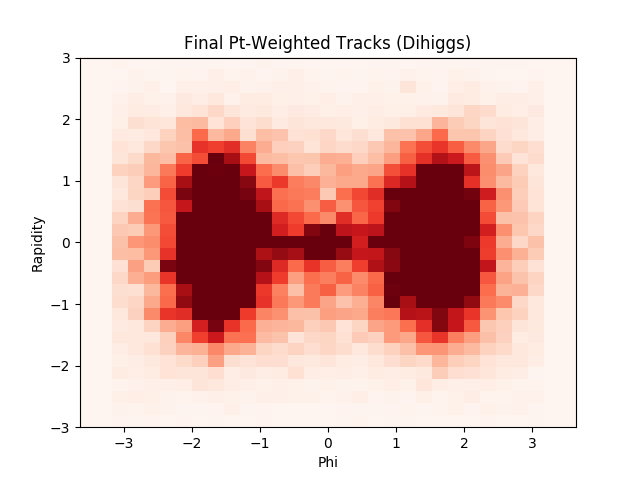
\includegraphics[width = 2in]{CNN/figures/images/qcd/Tracks_Dihiggs_Final_Pt-Weighted}} 
  \subfloat[]{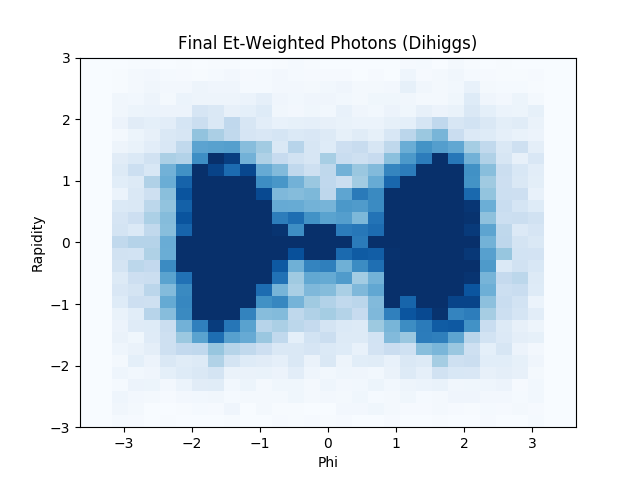
\includegraphics[width = 2in]{CNN/figures/images/qcd/Photons_Dihiggs_Final_Et-Weighted}}
  \subfloat[]{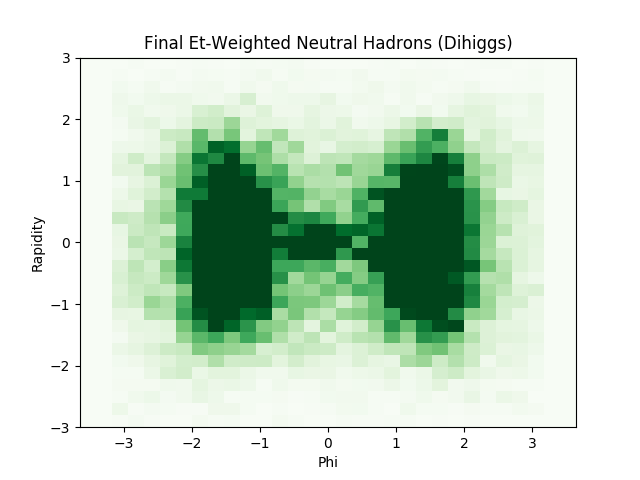
\includegraphics[width = 2in]{CNN/figures/images/qcd/NeutralHadrons_Dihiggs_Final_Et-Weighted}} \\
  \subfloat[]{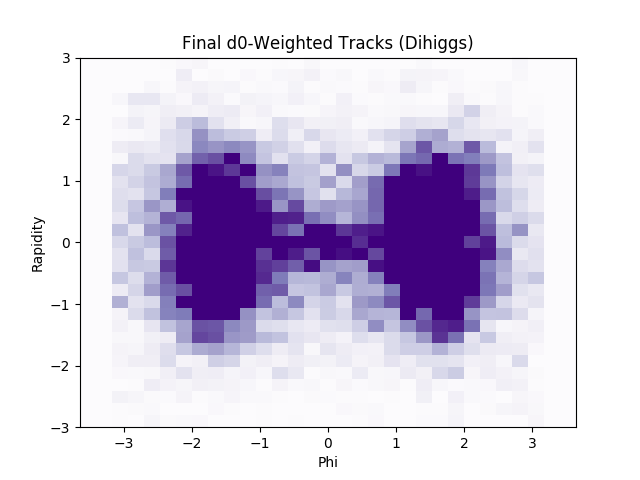
\includegraphics[width = 2in]{CNN/figures/images/qcd/Tracks_Dihiggs_Final_d0-Weighted}} 
  \subfloat[]{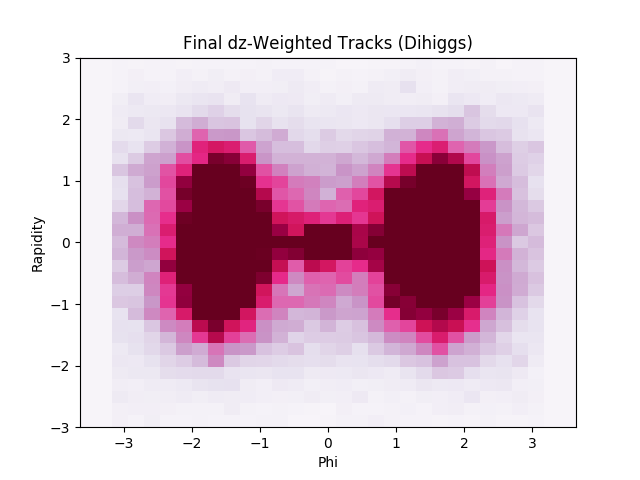
\includegraphics[width = 2in]{CNN/figures/images/qcd/Tracks_Dihiggs_Final_dz-Weighted}} 
\caption{Average QCD image showing (a) $p_{\textrm{T}}$-weighted tracks, (b) $E_{\textrm{T}}$-weighted ECAL deposits, (c) $E_{\textrm{T}}$-weighted HCAL deposits, (d) transverse impact parameter-weighted tracks, (e) longitudinal impact parameter-weighted tracks.}
\end{center}
\label{fig:cnn_avgQCD}
\end{figure}

\begin{figure}[!h] 
\begin{center}
  \subfloat[]{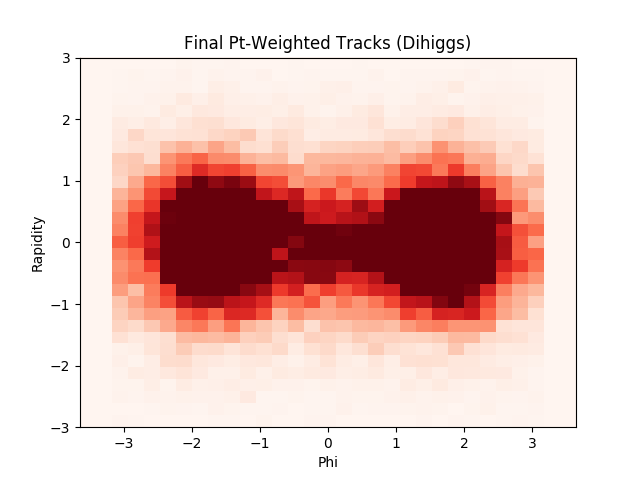
\includegraphics[width = 2in]{CNN/figures/images/hh/Tracks_Dihiggs_Final_Pt-Weighted}} 
  \subfloat[]{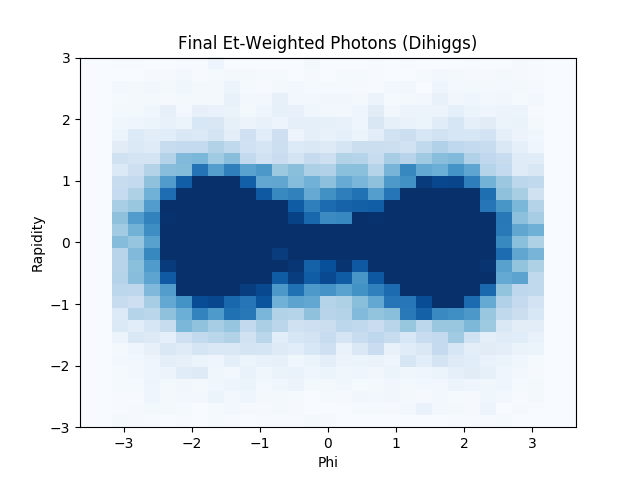
\includegraphics[width = 2in]{CNN/figures/images/hh/Photons_Dihiggs_Final_Et-Weighted}}
  \subfloat[]{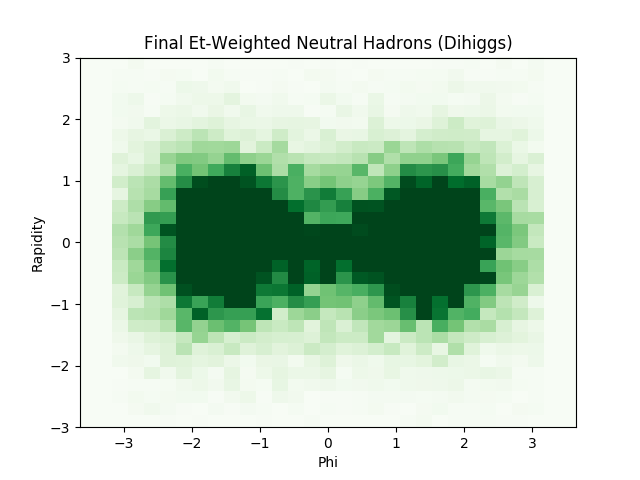
\includegraphics[width = 2in]{CNN/figures/images/hh/NeutralHadrons_Dihiggs_Final_Et-Weighted}} \\
  \subfloat[]{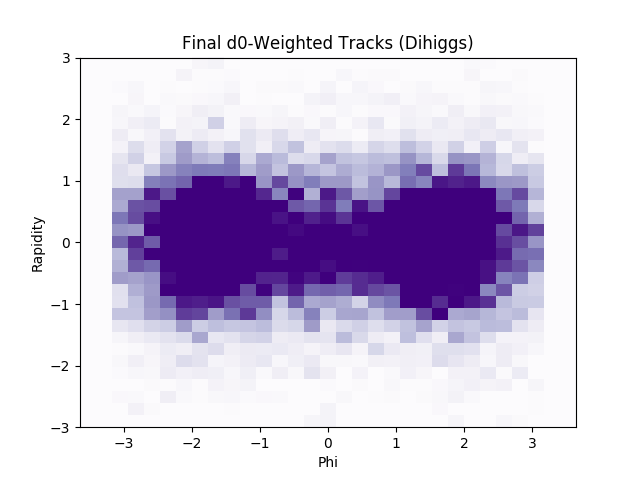
\includegraphics[width = 2in]{CNN/figures/images/hh/Tracks_Dihiggs_Final_d0-Weighted}} 
  \subfloat[]{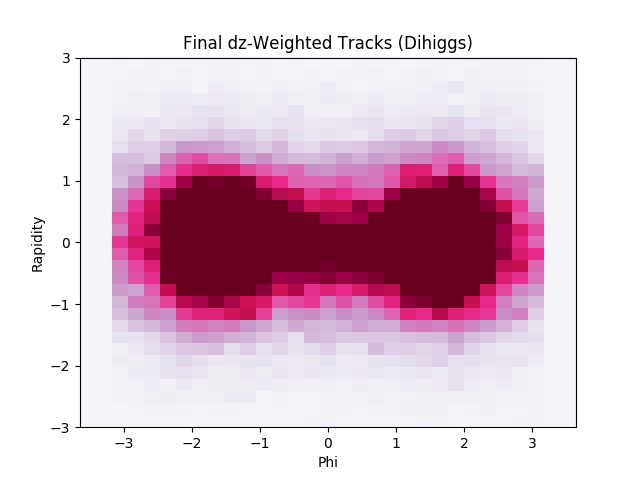
\includegraphics[width = 2in]{CNN/figures/images/hh/Tracks_Dihiggs_Final_dz-Weighted}} 
\caption{Average di-Higgs image showing (a) $p_{\textrm{T}}$-weighted tracks, (b) $E_{\textrm{T}}$-weighted ECAL deposits, (c) $E_{\textrm{T}}$-weighted HCAL deposits, (d) transverse impact parameter-weighted tracks, (e) longitudinal impact parameter-weighted tracks.}
\end{center}
\label{fig:cnn_avgDihiggs}
\end{figure}

As shown in Figures~\ref{fig:cnn_nominal} and \ref{fig:cnn_hybrid}, the CNN network structure uses two sequential 2D convolutional layers each with 16 3x3 filters, one max-pooling layer with a 2x2 window, a flattening of the outputs, two 64-node fully connected hidden layers, and one output layer for making the final prediction. As previously described, two of the networks append additional high level variables (scalar sum of transverse hadronic energy, number of jets, and number of $b$-tags) after the flattening and before the image information is fed through the fully connected layers. The optimal significance for each network is shown in Table~\ref{tab:cnnResults}. The best results were obtained using the 5-color network with additional high-level inputs, and the final predictions for this configuration are shown in Figure~\ref{fig:cnn_preds}. A best significance of 2.86$\pm$0.03 was found for a prediction cut $>$ 0.94 with a signal yield of 1.0$\cdot 10^4$ events and a background yield of 1.3$\cdot 10^7$ events.

\begin{table}[h!]
\label{tab:cnnResults}
  \begin{center}
    \begin{tabular}{|l|c|c|} % <-- Alignments: 1st column left, 2nd middle and 3rd right, with vertical lines in between
      \hline\hline
      \textbf{Method} & Best $S/\sqrt{B}$ & AUC \\
      \hline
      Tracks+HCAL+ECAL & 1.77 $\pm$ 0.01 & 0.818 \\
      Tracks+HCAL+ECAL + high-level & 2.12 $\pm$ 0.01 & 0.846 \\
      Tracks+HCAL+ECAL+D0+DZ & 2.45 $\pm$ 0.02 & 0.863 \\
      Tracks+HCAL+ECAL+D0+DZ + high-level & 2.86 $\pm$ 0.03 & 0.882 \\

      \hline\hline
    \end{tabular}
    \caption{Normalized to full HL-LHC dataset of 3000 fb$^{-1}$}
  \end{center}
\end{table}


\begin{figure}[!h] 
\begin{center}
  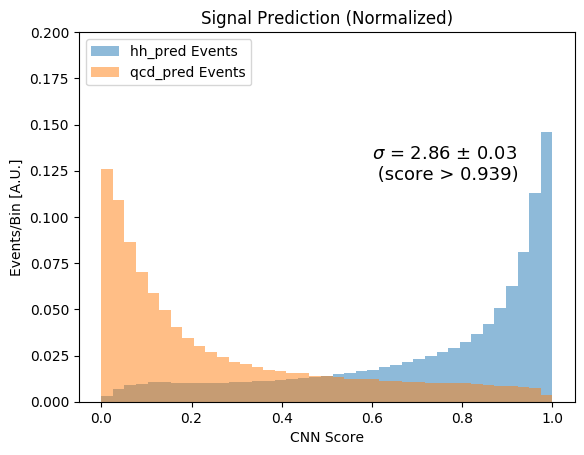
\includegraphics[width = 3in]{CNN/figures/5color_0PU_pix31_addHT-nJets-nBTags_2Conv16-16_one2DPool_EqualSamples/signal_CNNScore_norm}
  %\subfloat[]{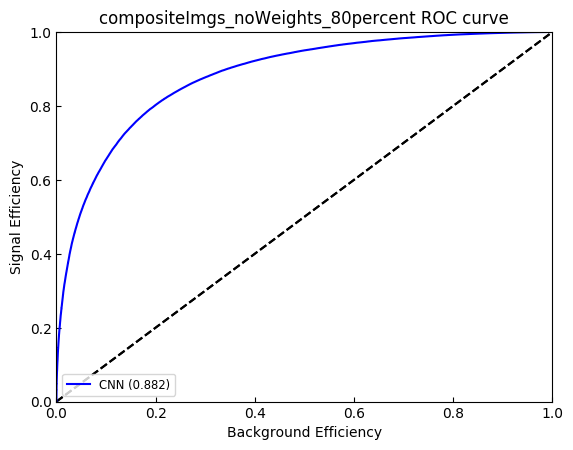
\includegraphics[width = 3in]{CNN/figures/5color_0PU_pix31_addHT-nJets-nBTags_2Conv16-16_one2DPool_EqualSamples/compositeImgs_noWeights_80percent_ROC}}\\
\caption{Signal prediction for the 5-color convolutional network with additional high-level inputs. The total area of the signal and background predictions are normalized to unity for easier shape comparison.}
\end{center}
\label{fig:cnn_preds}
\end{figure}



%\subsection{Residual Network}

%\subsection{Lorentz Boost Network}
%\label{sec:LBN}
a lorentz boost network? sounds cool, what's that?


% EFN network
\subsection{Energy Flow Network}
\label{sec:EFN}
Energy Flow Networks (EFN) and Particle Flow Networks (PFN) are algorithms that take basic jet constituents information as input rather than reconstructed jets and multi-jet composites, e.g. Higgs candidates. The EFN structure takes only the rapidity ${y}$ and azimuthal angle ${\phi}$ of jet constituents as input, while the PFN takes the rapidity $y$, azimuthal angle $\phi$, and transverse momentum $p_{T}$ of jet constituents as input. Using the constituents as input means no high level reconstruction is necessary when identifying events. Both the EFN and PFN are two-component networks, and their internal structures are shown in Figure \ref{fig:EFNArch}. The implementations of the EFN and PFN used for di-Higgs classification use 200 nodes for each hidden layer in network (a), 256 for latent space dimension and 300 nodes for each hidden layer in network (b). 

\begin{figure}[ht!]
\centering
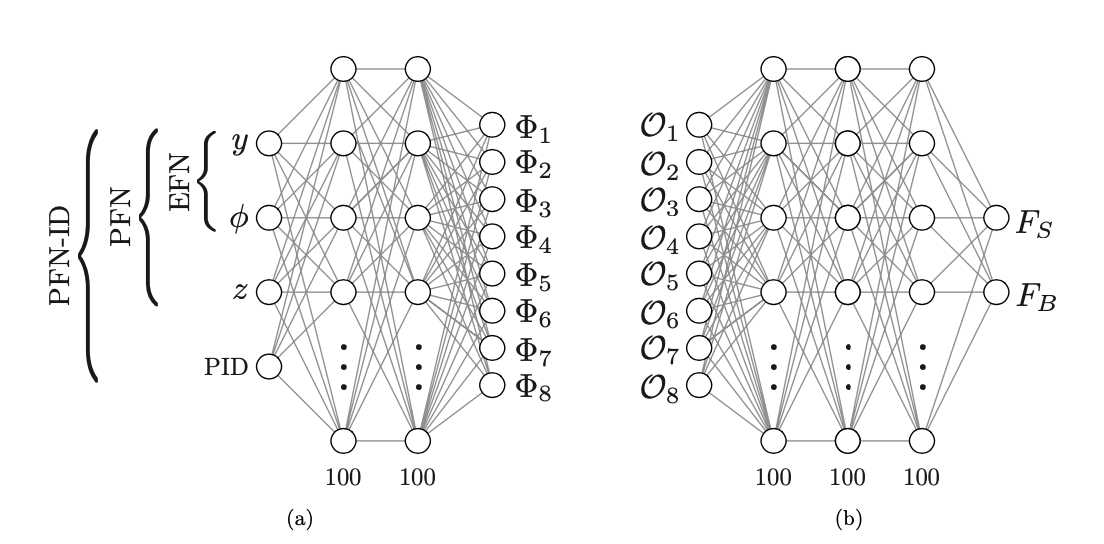
\includegraphics[scale=0.5]{./EFN/EFNArch.png}
\caption{Network (a) takes jet constituents information as input and outputs latent space $\Phi$ for each jet constituents. Network (b) takes $\mathcal{O}$, which is the linear combination of $\Phi$, as input and outputs final result.}
\label{fig:EFNArch}
\end{figure}

The EFN/PFN networks were trained using four separate categories split by number of jets and number of $b$-tags in order to test the network's dependence on higher-level jet information. Independent networks were trained using: all events, only events with $\geq$4 jets, only events with $\geq$4 jets and =2 $b$-tags, and only events with $\geq$4 jets and $\geq$4 $b$-tags. In each configuration, the number of signal and background events were adjusted to maintain an equal proportion of each population in the training sample. L2 regularization and dropout layers were added to minimize over-fitting. The results obtained with the EFN are shown in Table~\ref{EFNtab}. The results of the PFN are shown in Table~\ref{PFNtab}.

\begin{table}[ht!]
\centering
  %\begin{center}
    \begin{tabular}{|l|c|c|c|} % <-- Alignments: 1st column left, 2nd middle and 3rd right, with vertical lines in between
      \hline\hline
      \multirow{2}{*}{\textbf{Category}} & \multicolumn{3}{c|}{0PU}\\
      \cline{2-4}
      & Best $S/\sqrt{B}$ & \textbf{N$_{\mathrm{Signal}}$} & \textbf{N$_{\mathrm{Background}}$} \\
      \hline
      All Events & $1.407 \pm 0.006$ & $1.89\cdot 10^4$ & $1.80\cdot 10^8$ \\
      4Jets & $1.363 \pm 0.006$ & $1.63\cdot 10^4$ & $1.43\cdot 10^8$ \\
      4Jets 2BTags & $1.343 \pm 0.006$ & $1.33\cdot 10^4$ & $9.95\cdot 10^7$ \\
      4Jets 4BTags & $0.867 \pm 0.008$ & $3468.65$ & $1.60\cdot 10^7$ \\
      \hline\hline
    \end{tabular}
    \caption{EFN results. Normalized to full HL-LHC dataset of 3000 fb$^{-1}$}
  %\end{center}
\label{EFNtab}
\end{table}

\begin{table}[ht!]
\centering
  %\begin{center}
    \begin{tabular}{|l|c|c|c|} % <-- Alignments: 1st column left, 2nd middle and 3rd right, with vertical lines in between
      \hline\hline
      \multirow{2}{*}{\textbf{Category}} & \multicolumn{3}{c|}{0PU}\\
      \cline{2-4}
      & Best $S/\sqrt{B}$ & \textbf{N$_{\mathrm{Signal}}$} & \textbf{N$_{\mathrm{Background}}$} \\
      \hline
      All Events & $1.618 \pm 0.008$ & $1.79\cdot 10^4$ & $1.21\cdot 10^8$ \\
      4Jets & $1.580 \pm 0.008$ & $1.32\cdot 10^4$ & $7.00\cdot 10^7$ \\
      4Jets 2BTags & $1.574 \pm 0.009$ & $1.32\cdot 10^4$ & $4.85\cdot 10^7$ \\
      4Jets 4BTags & $0.903 \pm 0.009$ & $3297.34$ & $1.33\cdot 10^7$ \\
      \hline\hline
    \end{tabular}
    \caption{PFN results. Normalized to full HL-LHC dataset of 3000 fb$^{-1}$}
  %\end{center}
\label{PFNtab}
\end{table}

Both networks performed best when trained over all events without any cuts on the number of jets or $b$-tags. The EFN obtained a highest significance of 1.41$\pm$0.01, and the PFN obtained a highest significance of 1.62$\pm$0.01.



\section{Semi-Supervised Learning}
\label{sec:semisupervised}

\subsection{Clustering}
\label{sec:clusters}
k-means. Other? PCA?


\subsection{Auto-encoders}
\label{sec:AE}

An autoencoder (AE) is an unsupervised machine learning architecture used for detecting anomalies that differ significantly from the data used to train the network. The structure of the AE compresses the input information into a lower-dimensional representation called the latent space. This compression `encodes' the most important features of the training data into the latent space, while the second half of the network `decodes' the latent space back into a representation approaching the original inputs.

This construction fundamentally changes the meaning of the loss calculation-- rather than computing the loss between a prediction and a target, the AE loss is a measure of how well the network reproduces the original inputs after encoding and decoding. Inputs that differ significantly from the data used to train the AE will not be properly reconstructed, and anomalies can be identified by selecting events with large losses. Training with Monte Carlo simulations allows for a semi-supervised cross-check on AE performance since the classes of training and testing samples are known in advance.

Because AE anomaly detection relies on a well-modeled understanding of background processes, the network was trained using only QCD events. Additional models were trained by substituting the pure-QCD training sample with training samples consisting of mixtures of QCD and di-Higgs events to test the stability of the method against signal contamination. No significant deterioration was observed for reasonable levels of contamination. The AE used for di-Higgs detection was built using the Keras package~\cite{chollet2015keras} and consists of an input layer, a single hidden layer, and an output layer. Eleven reconstructed variables were selected for use in the AE. 

\begin{figure}[!h] 
\begin{center}
\includegraphics*[width=0.75\textwidth] {AE/figures/ae_PCA_11vars}
\caption{PCA performed on the selected eleven kinematic inputs. The x-axis indicates the number of PCA features, and the y-axis indicates the variance. Choosing the optimal size for the latent space requires identifying the point of diminishing variance return.}
  \label{fig:ae_pca}
\end{center}
\end{figure}

The output layer is a mirror of the input layer and therefore has 11 nodes. A PCA analysis (shown in Figure~\ref{fig:ae_pca}) was used to determine that a latent space of three nodes was optimal. The hidden layer and output layer use ReLU and sigmoid activation functions respectively. An L2 regularization term was added to the hidden layer to avoid over-fitting. %Afterwards the model was compiled using the ‘adam’ optimizer with the mean-squared error loss. Finally, the model was fit on the training data along with the validation data for 10000 epochs. The ‘EarlyStopping’ function was used to shorten training time by stopping training after the validation accuracy didn’t increase by 0.001 for 50 epochs. The batch size during training was set to 1024 in order to both decrease training time and prevent overfitting.
Because training an autoencoder is an unsupervised and unlabeled process, there is no prediction of whether a given event is signal or background. Since di-Higgs events should be relatively anomalous compared to the QCD training set, signal events should have a relatively larger average loss value. Cutting on the loss function allows for a significance to be calculated for comparison with other methods.

\begin{figure}[!h] 
  \begin{center}
    \subfloat[]{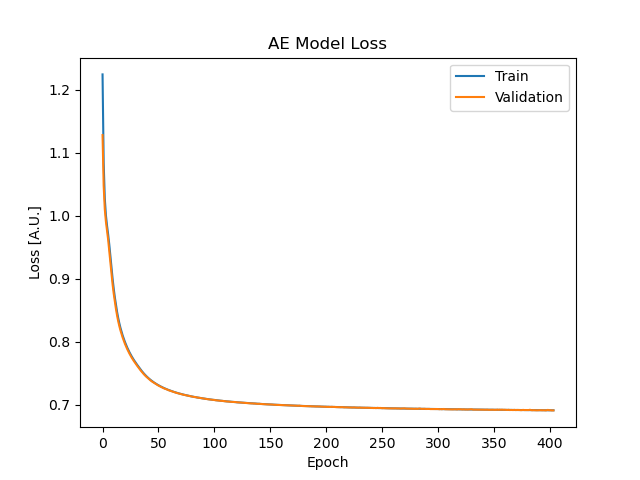
\includegraphics[width = 3in]{AE/figures/ae_modelLoss_qcdTrain_v2}} 
    \subfloat[]{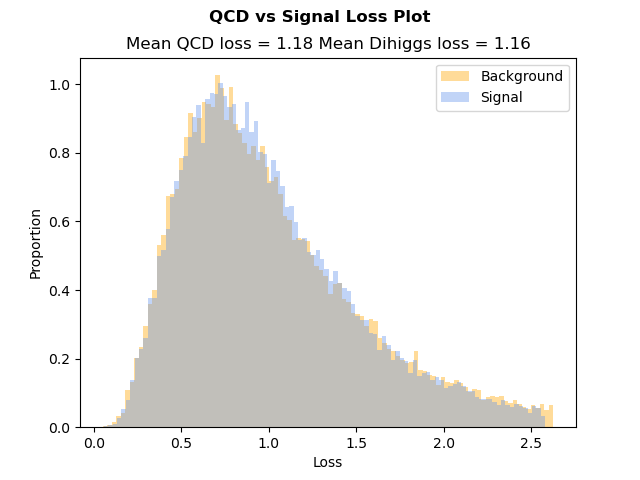
\includegraphics[width = 3in]{AE/figures/ae_finalLossDistribution_qcdTrain_v2}}\\
    \caption{(Left) The loss of the AE during QCD training/reconstruction converged after 700 epochs. (Right) The loss distribution generated by the AE when being tested on QCD and di-Higgs event data separately.}    
  \label{fig:ae_trainPredLoss}
\end{center}
\end{figure}

Training for several hundred epochs leads the model to converge, and it reaches an asymptotic loss value near 0.7 (see Figure~\ref{fig:ae_trainPredLoss}). Requiring the loss to be larger than 0.05 yields a best significance of $\sigma$ = 0.81$\pm$0.01. This significance value may be somewhat misleading since the signal and background loss distributions have little separation. The highest significance result effectively is a cut that keeps nearly all events. This suggests that the kinematic inputs used in training do not significantly differ between signal and background processes after the latent space compression.

%\begin{figure}[!h] 
%\begin{center}
%\includegraphics*[width=0.75\textwidth] {AE/figures/ae_finalSignalPredictions_qcdTrain}
%\caption{Signal predictions made by the AE based on the loss distributions from Fig. 3. The $S/\sqrt{B}$ best cut was placed near 0.1, indicating that the AE was not able to sufficiently distinguish di-Higgs da%ta from QCD data.}
%  \label{fig:ae_signalPred}
%\end{center}
%\end{figure}



\section{Results}
\label{sec:results}

The methods covered in this paper are by no means an exhaustive review of the ML landscape available to high energy physics. Still, a wide range of techniques and philosophies are covered. Table~\ref{tab:summary} provides a summary of the methods described in the previous sections. The results of a traditional 1-D sequential cut technique is shown for comparison though the details have not been discussed in the previous sections. Clear gains in sensitivity compared to this baseline are apparent for many of the ML models tested in this review.

\begin{table}[h!]
\label{tab:summary}
  \begin{center}
  \begin{tabular}{|l|c|c|c|} % <-- Alignments: 1st column left, 2nd middle and 3rd right, with vertical lines in between
      \hline\hline
      \multirow{2}{*}{\textbf{Method}} & \multicolumn{3}{c|}{0PU} \\
      \cline{2-4}
      & Best $\sigma$ & \textbf{N$_{\mathrm{Signal}}$} & \textbf{N$_{\mathrm{Background}}$} \\
      \hline
      Autoencoder           & 0.81 $\pm$ 0.01 & 5840.8 & 5.2 $\cdot$ $10^7$ \\
      1D-Rectangular Cuts   & 0.82 $\pm$ 0.02 & 3621.0 & 1.97 $\cdot$ $10^7$ \\
      k-Means Clustering    & 1.44 $\pm$ 0.02 & 1703.6 & 1.4 $\cdot$ $10^6$ \\
      Particle Flow Network & 1.62 $\pm$ 0.01 & 1.8 $\cdot$ $10^4$ & 1.2 $\cdot$ $10^8$ \\
      Boosted Decision Tree & 1.84 $\pm$ 0.09 & 986.3  & 2.8 $\cdot$ $10^5$ \\
      %Lorentz Boost Network & 1.87 $\pm$ 0.08 & 1123.3 & 3.6 $\cdot$ $10^5$ \\
      Feed-Forward NN       & 2.40 $\pm$ 0.08 & 1659.9 & 4.8 $\cdot$ $10^5$ \\
      Random Forest         & 2.44 $\pm$ 0.19 & 544.7 & 5.0 $\cdot$ $10^4$ \\
      Convolutional NN      & 2.85 $\pm$ 0.02 & 1.0 $\cdot$ $10^4$ & 1.3 $\cdot$ $10^7$ \\
      \hline\hline
    \end{tabular}
    \caption{Comparison of method significance and signal/background yields normalized to full HL-LHC dataset of 3000 fb$^{-1}$.}
  \end{center}
\end{table}

An important caveat to keep in mind is that all results discussed here were determined in conditions with zero pileup. In higher pileup environments like those expected at the HL-LHC, reconstruction algorithms see serious reductions in correct combinatoric matching. This effect will certainly degrade the expected performance of techniques that rely on explicit event reconstruction. Methods that do not rely on event reconstruction (CNN, PFN) might be more robust to these effects, and this should be studied in further work. The unsupervised AE technique performed the worst among all the methods tested, but this is likely a reflection of the fact that model-specific methods often outperform model-unspecific methods when evaluated on the model used in training.



\section{Conclusions}
\label{sec:conclusions}
Measuring the rate of dihiggs production will be a problem facing the high energy physics community through the end of the HL-LHC era. The techniques explored in this paper show the power of machine learning techniques to identify dihiggs signals from amongst overwhelming QCD signals. The significance obtained for many of these methods is impressive given the simplicity of the evaluation metric and bodes well for current and future measurements of double higgs production at the LHC.




% Extra stuff
%\acknowledgments

This is the most common positions for acknowledgments. A macro is
available to maintain the same layout and spelling of the heading.

\paragraph{Note added.} This is also a good position for notes added
after the paper has been written.


%\backmatter
% We use BIBTeX for the bibliography---you don't have to
%% The bibliography will probably be heavily edited during typesetting.
% We'll parse it and, using the arxiv number or the journal data, will
% query inspire, trying to verify the data (this will probalby spot
% eventual typos) and retrive the document DOI and eventual errata.
% We however suggest to always provide author, title and journal data:
% in short all the informations that clearly identify a document.

\begin{thebibliography}{99}

\bibitem{a}
Author, \emph{Title}, \emph{J. Abbrev.} {\bf vol} (year) pg.

\bibitem{b}
Author, \emph{Title},
arxiv:1234.5678.

\bibitem{c}
Author, \emph{Title},
Publisher (year).


% Please avoid comments such as "For a review'', "For some examples",
% "and references therein" or move them in the text. In general,
% please leave only references in the bibliography and move all
% accessory text in footnotes.

% Also, please have only one work for each \bibitem.


\end{thebibliography}


\nocite{*} % To display all refs, even uncited refs (useful when editting)
%\bibliography

\cleardoublepage
\phantomsection

%\addcontentsline{toc}{chapter}{Bibliography}
\bibliographystyle{ieeetr}
\bibliography{bibliography}

%\bibliographystyle{unsrt} % use your favorite BIBTeX style

% APPENDICES IF NEEDED
%\appendix
\section{First Appendix}
Please always give a title also for appendices.



\end{document}
